
%%%%%%%%%%%%%%%%%%%%%%%%%%%%%%%%%%%%%%%%%%%%%%%%%%%%%%%%
%
% Copyright (c) 2003-2011 by University of Queensland
% Earth Systems Science Computational Center (ESSCC)
% http://www.uq.edu.au/esscc
%
% Primary Business: Queensland, Australia
% Licensed under the Open Software License version 3.0
% http://www.opensource.org/licenses/osl-3.0.php
%
%%%%%%%%%%%%%%%%%%%%%%%%%%%%%%%%%%%%%%%%%%%%%%%%%%%%%%%%

\section{3D pycad}
\sslist{example09m.py}
This example explains how to build a 3D layered domain using pycad. As
simple as this example sounds, there are a few import concepts that one must
remember  so that the model will function correctly.
\begin{itemize}
  \item There must be no duplication of any geometric features whether they are
  points, lines, loops, surfaces or volumes.
  \item All objects with dimensions greater then a line have a normal defined by
  the right hand rule (RHR). It is important to consider which direction a
  normal is oriented when combining primitives to form higher order shapes.
\end{itemize}

The first step as always is to import the external modules. To build a 3D model
and mesh we will need pycad, some GMesh interfaces, the Finley domain builder
and some additional tools.
\begin{python}
#######################################################EXTERNAL MODULES
from esys.pycad import * #domain constructor
from esys.pycad.gmsh import Design #Finite Element meshing package
from esys.finley import MakeDomain #Converter for escript
from esys.escript import mkDir, getMPISizeWorld
import os
\end{python}
After carrying out some routine checks and setting the \verb!save_path! we then
specify the parameters of the model. This model will be 2000 by 2000 meters on
the surface and extend to a depth of 500 meters. An interface or boundary
between two layers will be created at half the total depth or 250 meters. This
type of model is known as a horizontally layered model or a layer cake model. 
\begin{python}
################################################ESTABLISHING PARAMETERS
#Model Parameters
xwidth=2000.0*m   #x width of model
ywidth=2000.0*m   #y width of model
depth=500.0*m   #depth of model
intf=depth/2.   #Depth of the interface.
\end{python}
We now start to specify the components of our model starting with the vertexes
using the \verb!Point! primitive. These are then joined by lines in a regular
manner taking note of the right hand rule. Finally, the lines are turned into
loops and then planar surfaces.
\footnote{Some code has been emmitted here for
simlpicity. For the full script please refer to the script referenced at the beginning of
this section.}
\begin{python}
####################################################DOMAIN CONSTRUCTION
# Domain Corners
p0=Point(0.0,    0.0,      0.0)
#..etc..
l45=Line(p4, p5)

# Join line segments to create domain boundaries and then surfaces
ctop=CurveLoop(l01, l12, l23, l30);     stop=PlaneSurface(ctop)
cbot=CurveLoop(-l67, -l56, -l45, -l74); sbot=PlaneSurface(cbot)
\end{python}
With the top and bottom of the domain taken care of, it is now time to focus on
the interface. Again the vertexes of the planar interface are created. With
these, vertical and horizontal lines (edges) are created joining the interface
with itself and the top and bottom surfaces. 
\begin{python}
# for each side
ip0=Point(0.0,    0.0,      intf)
#..etc..
linte_ar=[]; #lines for vertical edges
linhe_ar=[]; #lines for horizontal edges
linte_ar.append(Line(p0,ip0))
#..etc..
linhe_ar.append(Line(ip3,ip0))
\end{python}
Consider now the sides of the domain. One could specify the whole side using the
points first defined for the top and bottom layer. This would define the whole
domain as one volume. However, there is an interface and we wish to define each
layer individually. Therefore, there will be 8 surfaces on the sides of our
domain. We can do this operation quite simply using the points and lines that we
had defined previously. First loops are created and then surfaces making sure to
keep a normal for each layer which is consistent with upper and lower surfaces
of the layer. For example, all surface normals must face outwards from or
inwards towards the centre of the volume.
\begin{python}
cintfa_ar=[]; cintfb_ar=[] #curveloops for above and below interface on sides
cintfa_ar.append(CurveLoop(linte_ar[0],linhe_ar[0],-linte_ar[2],-l01))
#..etc..
cintfb_ar.append(CurveLoop(linte_ar[7],l45,-linte_ar[1],-linhe_ar[3]))

sintfa_ar=[PlaneSurface(cintfa_ar[i]) for i in range(0,4)]
sintfb_ar=[PlaneSurface(cintfb_ar[i]) for i in range(0,4)]

sintf=PlaneSurface(CurveLoop(*tuple(linhe_ar)))
\end{python}
Assuming all is well with the normals, the volumes can be created from our
surface arrays. Note the use here of the \verb!*tuple! function. This allows us
to pass an list array as an argument list to a function. It must be placed at
the end of the function arguments and there cannot be more than one per function
call.
\begin{python}
vintfa=Volume(SurfaceLoop(stop,-sintf,*tuple(sintfa_ar)))
vintfb=Volume(SurfaceLoop(sbot,sintf,*tuple(sintfb_ar)))

# Create the volume.
#sloop=SurfaceLoop(stop,sbot,*tuple(sintfa_ar+sintfb_ar))
#model=Volume(sloop)
\end{python}
The final steps are designing the mesh, tagging the volumes and the interface
and outputting the data to file so it can be imported by an \esc solution
script.
\begin{python}
#############################################EXPORTING MESH FOR ESCRIPT
# Create a Design which can make the mesh
d=Design(dim=3, element_size=5.0*m)
d.addItems(PropertySet('vintfa',vintfa))
d.addItems(PropertySet('vintfb',vintfb))
d.addItems(sintf)

d.setScriptFileName(os.path.join(save_path,"example09m.geo"))

d.setMeshFileName(os.path.join(save_path,"example09m.msh"))
#
#  make the finley domain:
#
domain=MakeDomain(d)
# Create a file that can be read back in to python with
# mesh=ReadMesh(fileName)
domain.write(os.path.join(save_path,"example09m.fly"))
\end{python}

\begin{figure}[htp]
\begin{center}
\begin{subfigure}[Gmesh view of geometry only.]
{\label{fig:gmsh3dgeo}
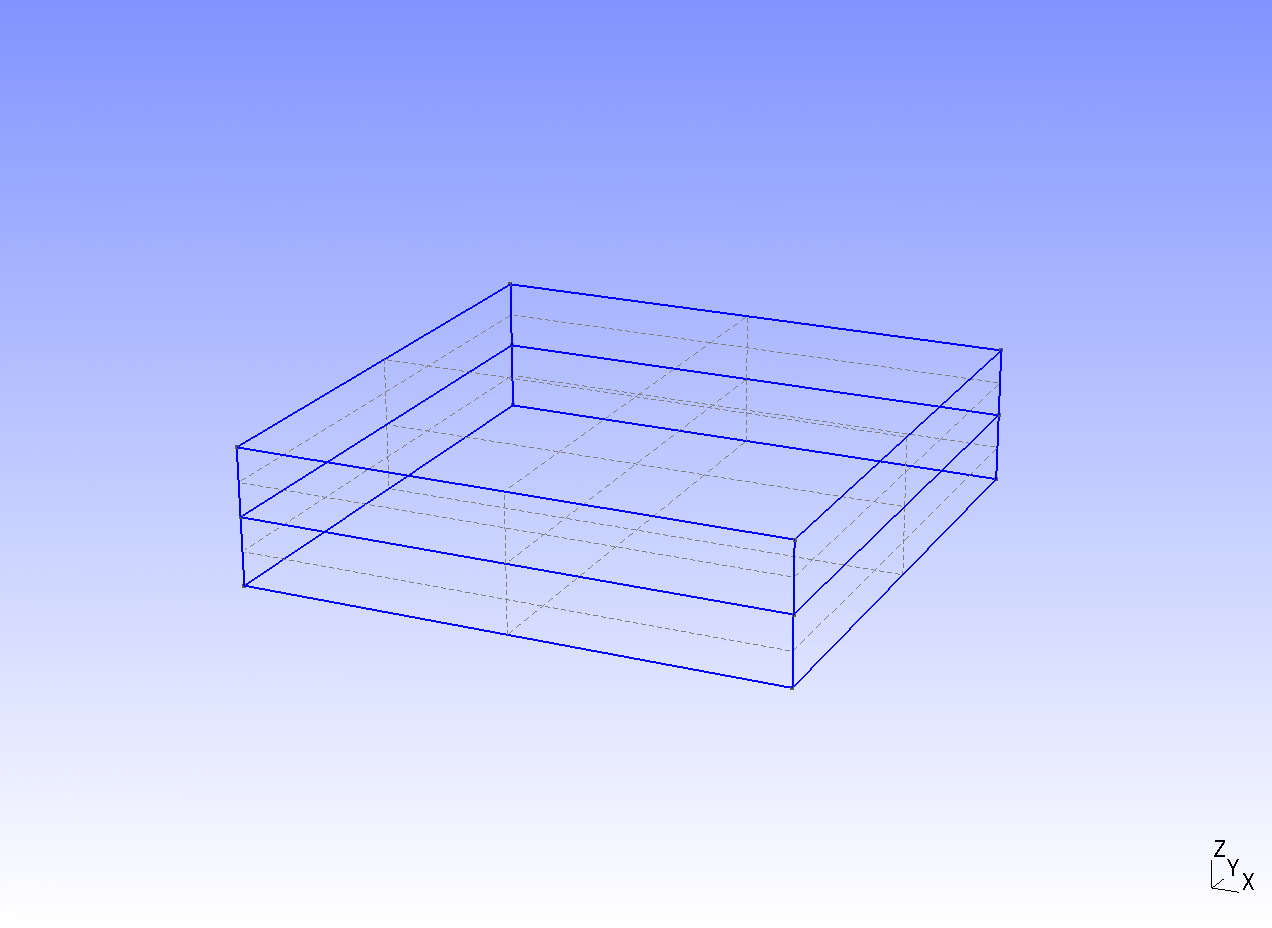
\includegraphics[width=3.5in]{figures/gmsh-example09m.png}}
\end{subfigure}
\begin{subfigure}[Gmesh view of a 200m 2D mesh on the domain surfaces.]
{\label{fig:gmsh3dmsh}
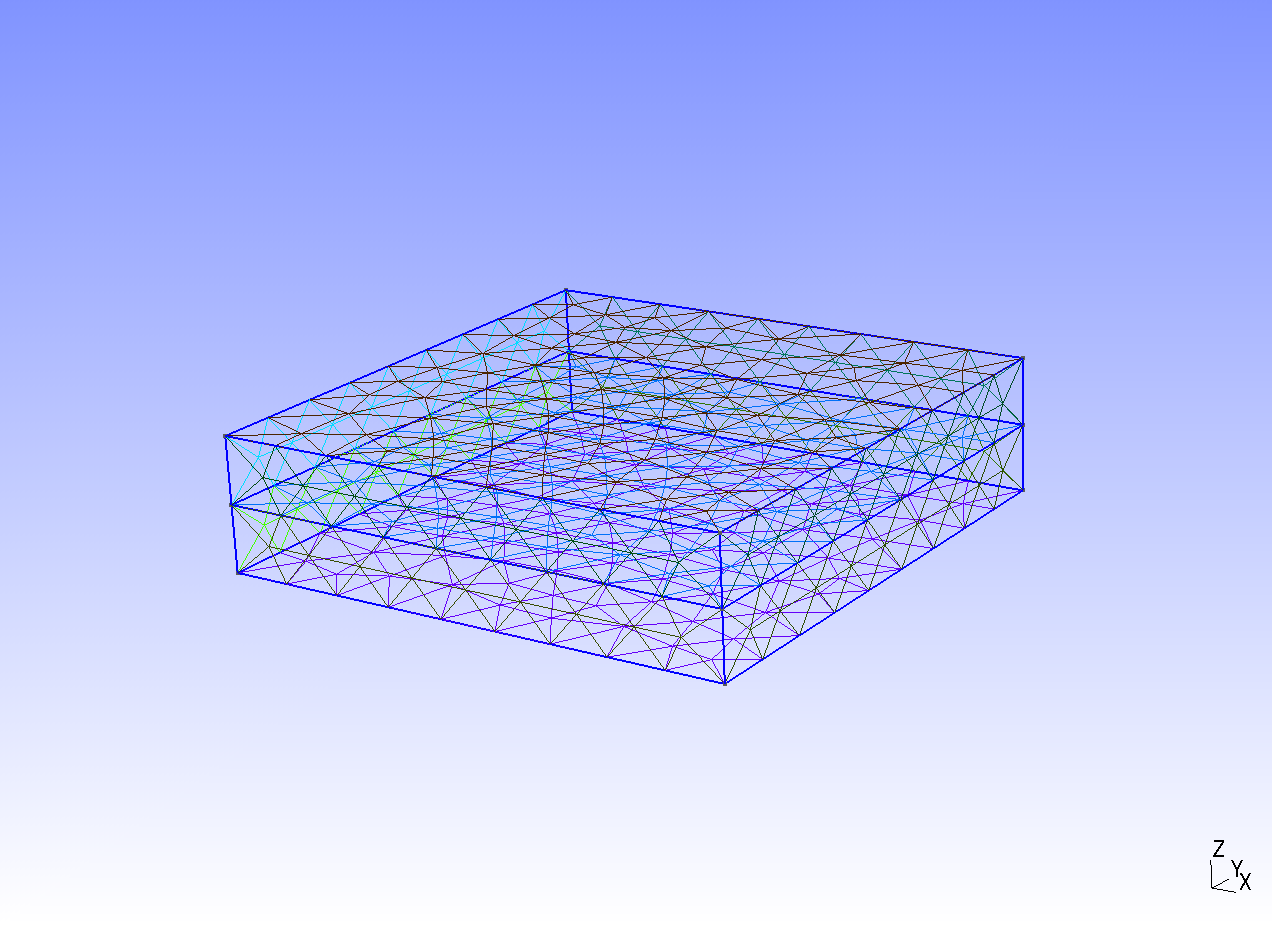
\includegraphics[width=3.5in]{figures/gmsh-example09msh2d.png}}
\end{subfigure}
\begin{subfigure}[Gmesh view of a 200m 3D mesh on the domain volumes.]
{\label{fig:gmsh3dmsh}
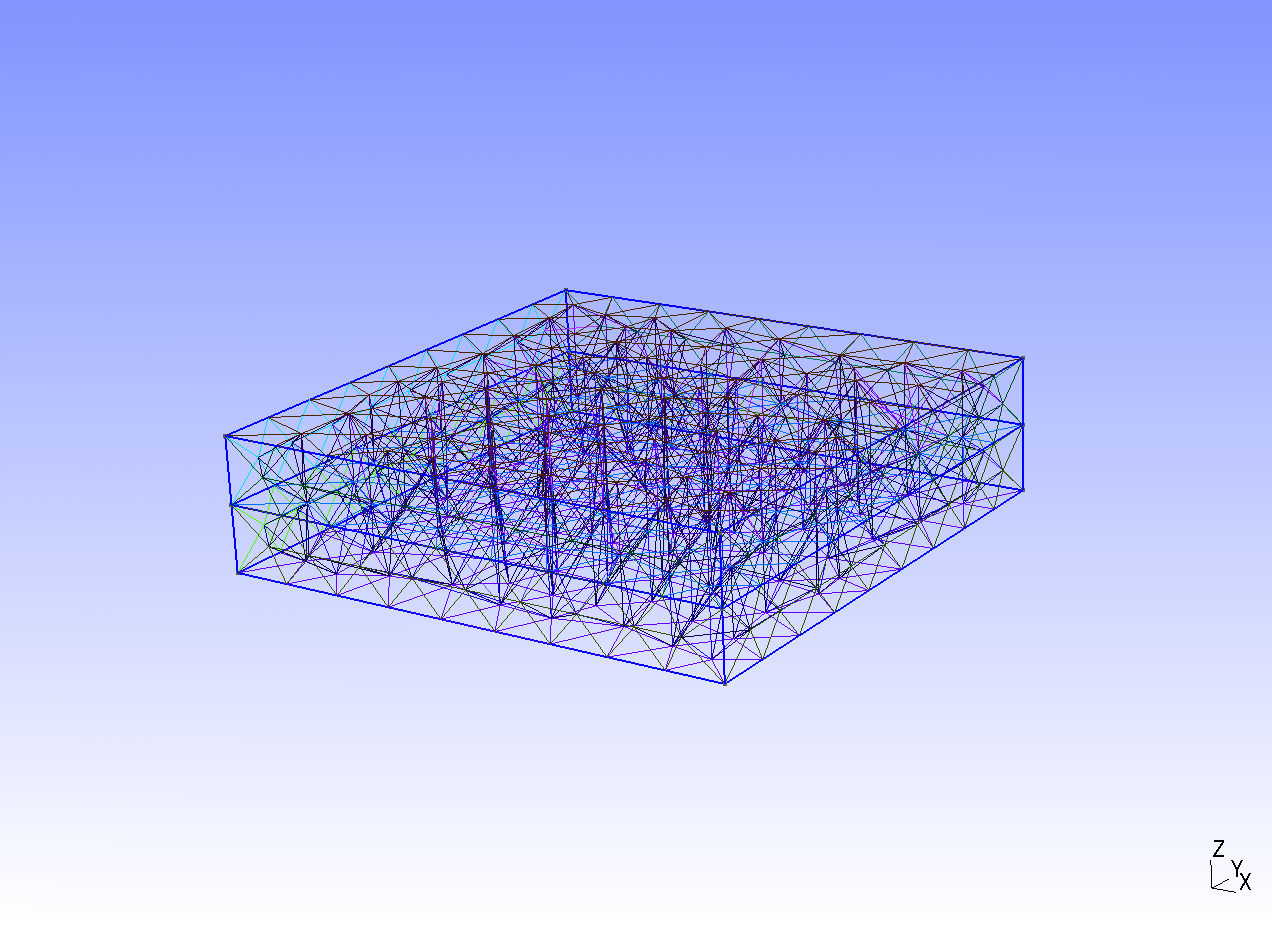
\includegraphics[width=3.5in]{figures/gmsh-example09msh3d.png}}
\end{subfigure}
\end{center}
\end{figure}
\clearpage

\section{Layer Cake Models}
Whilst this type of model seems simple enough to construct for two layers,
specifying multiple layers can become cumbersome. A function exists to generate
layer cake models called \verb!layer_cake!. A detailed description of its
arguments and returns is available in the API and the function can be imported
from the pycad.extras module.
\begin{python}
from esys.pycad.extras import layer_cake
intfaces=[10,30,50,55,80,100,200,250,400,500]

domaindes=Design(dim=3,element_size=element_size,order=2)
cmplx_domain=layer_cake(domaindes,xwidth,ywidth,intfaces)
cmplx_domain.setScriptFileName(os.path.join(save_path,"example09lc.geo"))
cmplx_domain.setMeshFileName(os.path.join(save_path,"example09lc.msh"))
dcmplx=MakeDomain(cmplx_domain)
dcmplx.write(os.path.join(save_path,"example09lc.fly"))
\end{python}

\begin{figure}[ht]
\begin{center}
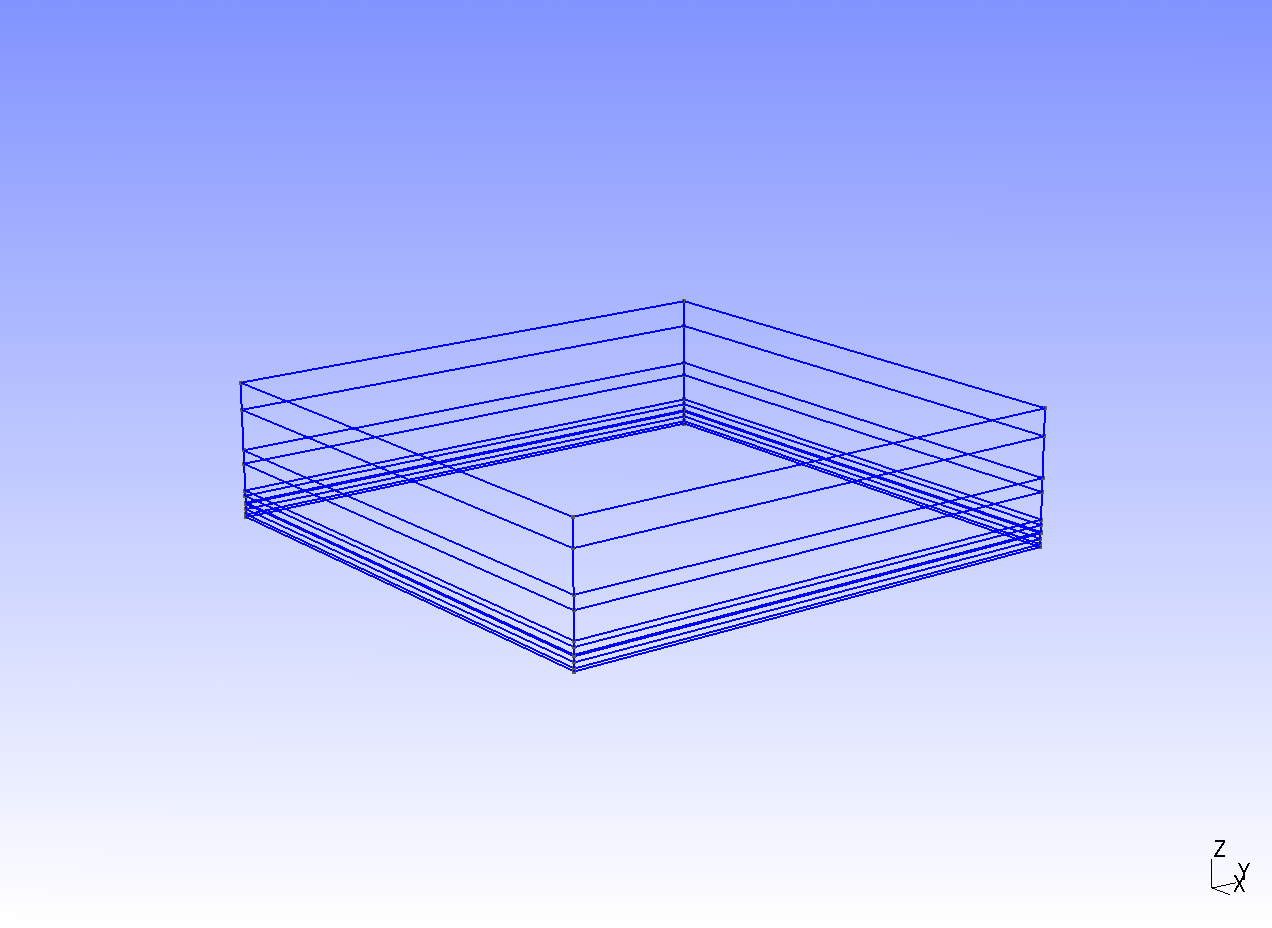
\includegraphics[width=5in]{figures/gmsh-example09lc.png}
\caption{Example geometry using layer cake function.}
\label{fig:gmsh3dlc}
\end{center}
\end{figure}
\clearpage
\section{Troubleshooting Pycad}
There are some techniques which can be useful when trying to troubleshoot
problems with pycad. As mentioned earlier it is important to ensure the correct
directionality of your primitives when constructing more complicated domains. If
it remains too difficult to establish the tangent of a line or curveloop, or
the normal of a surface, these values can be checked by importing the geometry
to gmesh and applying the appropriate visualisation options.

\section{3D Seismic Wave Propagation}
Adding an extra dimension to our wave equation solution script should be
relatively simple. Apart from the changes to the domain and therefore the
parameters of the model, there are only a few minor things which must be
modified to make the solution appropriate for 3d modelling.

\section{Applying a function to a domain tag}
\sslist{example09a.py}
To apply a function or data object to a domain requires a two step process. The
first step is to create a data object with an on/off mask based upon the tagged
value. This is quite simple and can be achieved by using a scalar data object
based upon the domain. In this case we are using the \verb!FunctionOnBoundary!
function space because the tagged value \verb!'stop'! is effectively a specific
subsurface of the boundary of the whole domain. 
\begin{python}
stop=Scalar(0.0,FunctionOnBoundary(domain))
stop.setTaggedValue("stop",1.0)
\end{python}
Now the data object \verb|stop| has the value 1.0 on the surface
\verb!'stop'! and zero everywhere else.
% 
 To apply our function to the boundary only on \verb|stop| we now
 mulitply it by \verb|stop|
\begin{python}
xb=FunctionOnBoundary(domain).getX()
yx=(cos(length(xb-xc)*3.1415/src_length)+1)*whereNegative(length(xb-xc)-src_length)
src_dir=numpy.array([0.,0.,1.0]) # defines direction of point source as down
mypde.setValue(y=source[0]*yx*src_dir*stop) #set the source as a function on the boundary
\end{python}

\section{Mayavi2 with 3D data.}
There are a variety of visualisation options available when using VTK data. The
types of visualisation are often data and interpretation specific and thus
consideration must be given to the type of output saved to file. Whether that is
scalar, vector or tensor data.

\begin{figure}[htp]
\centering
\begin{subfigure}[Example 9 at time step 201.]
 	{\label{fig:ex9b 201}
 	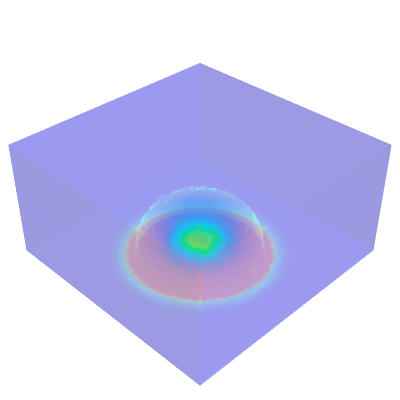
\includegraphics[width=0.45\textwidth]{figures/ex09b00201.png}}
 \end{subfigure}
 \begin{subfigure}[Example 9 at time step 341.]
 	{\label{fig:ex9b 201}
 	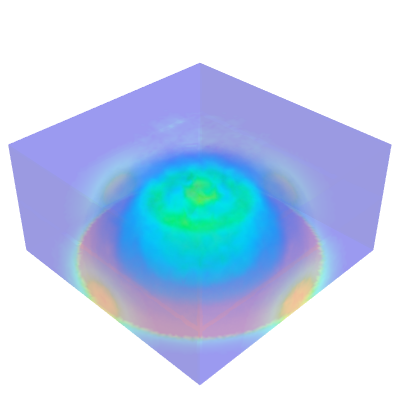
\includegraphics[width=0.45\textwidth]{figures/ex09b00341.png}}
 \end{subfigure}\\
 \begin{subfigure}[Example 9 at time step 440.]
 	{\label{fig:ex9b 201}
 	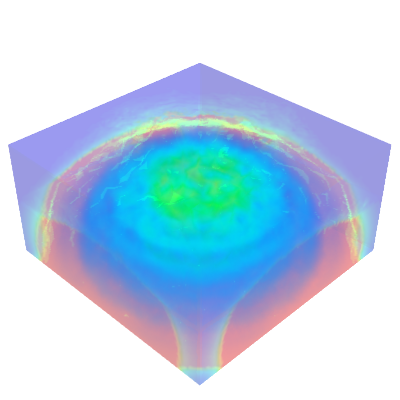
\includegraphics[width=0.45\textwidth]{figures/ex09b00440.png}}
 \end{subfigure}
\end{figure}
